\section{Subgroups}
When we talked about sets, we mentioned the notion of a subset. The idea of a substructure is not unique to the world of sets. We have subspaces of vector spaces, submanifolds of manifolds, and subgroups of groups. Groups are more complex structures that sets, however, and as a result the definition of a subgroup requires more detail than that of a subset.

\begin{definition}{Subgroup}
	Let $G$ be a group and let $H\subset G$. Then $H$ is a subgroup of $G$, written $H\leq G$ if
	\begin{enumerate}
		\item $H$ is closed under the operation on $G$
		\item The identity element in $G$ is contained within $H$.
		\item If $h\in H$, then $h^{-1}\in H$.
	\end{enumerate}
\end{definition}

The main idea to take away from this definition is that when we want to show something is a subgroup, we need to show containment; when we want to show something is a group, we need to show existence. Let's look at some properties of subgroups.

\begin{theorem}{}
	A set $H\subset G$ is a subgroup of $G$ if
	\begin{enumerate}
		\item $H\neq\emptyset$ and
		\item $a,b\in H\implies ab^{-1}\in H$.
	\end{enumerate}
\end{theorem}
\begin{proof}
	Since $H\neq\emptyset$, we know $a\in H\implies a^{-1}\in H$. Therefore $aa^{-1}=e\in H$. Finally, let $h_{1},h_{2}\in H$. Since $h_{2}\in H$, we have that $h_{2}^{-1}\in H$. Then $h_{1}(h_{2}^{-1})^{-1}\in H \implies h_{1}h_{2}\in H$.
	Hence, the group is closed, contains inverses, and contains the identity.
\end{proof}
This is often called the subgroup test, and is sometimes easier to use than the definition of subgroup when trying to prove something is a subgroup. Another property of subgroups unites the idea of a cyclic group and a subgroup.

\begin{theorem}{}\label{thm:cyclic_subgroup}
	Let $G$ be a cyclic group. Then $H\leq G\implies H$ is cyclic.
\end{theorem}
\begin{proof}
	Suppose $H\neq <e>$ and let $G=<a>$. We need to find a generator for $H$. Since $H\leq G$, we know that every element of $h$ can be written in the from $a^{n}$ for some $a\in G$ and some $n\in\NN$, so we consider $a^{d}$ where $d\in\NN$ where $d$ is the minimal element such that $a^{d}\in H$.
	We claim that $H=<a^{d}>$. To see this, let $b\in H$. Then $b$ can be written as $a^{n}$ as well. If we can show that $d\mid n$, then we will be done. Then
	\begin{align*}
		n     & = md+r\qquad 0\leq r\leq d-1 \\
		a^{n} & = a^{md+r}                   \\
		a^{n} & = a^{md}a^{r}\in H.
	\end{align*}
	Since $H\leq G$, we know that $a^{md}\in H\implies a^{-md}\in H$. Then
	\[
		a^{-md}a^{n}=a^{-md}a^{md}a^{r}\implies
		a^{n-md}=a^{r}\implies
		a^{r}\in H,
	\]
	but $r$ must be 0 since $d$ was the minimal element for which $a^{d}\in H$. Hence, we conclude that $a^{n}=a^{md}$, so $d\mid n$ and therefore $H=<a^{d}>$.
\end{proof}

This theorem is one of the reasons that we like cyclic groups so much; a common technique for proving something is a group is to prove that it's a subgroup of another group. If we could show that the parent group was cyclic, then we get the added bonus of our group being cyclic as well.

We are now ready to move onto one of the most powerful theorems of this chapter (it has a name, so it must be important). This particular theorem concerns the orders of subgroups.
\begin{theorem}{Theorem of Lagrange}\label{thm:lagrange}
	Let $G$ be a group and let $H\leq G$. Then $ord(H)\mid ord(G)$.
\end{theorem}
We are not ready to prove this theorem quite yet as it requires some knowledge of what are known as cosets. We can extrapolate some more interesting results from the theorem of Lagrange, such as the fact that
\begin{theorem}{}\label{thm:subgroup_m}
	Let $G$ be a cyclic group with $|G|=n$. Then if $\exists m\in G\suchthat m\mid ord(G)$, then $G$ has a subgroup of order $m$, and this subgroup is unique.
\end{theorem}
The theorem of Lagrange does not guarantee existence of subgroups, only that if such a subgroup exists, then the order must divide the group's order; \cref{thm:subgroup_m} guarantees us existence provided that the group is cyclic. In fact, we can even do a little better than \cref{thm:subgroup_m}.
\begin{corollary}
	If $G=<a>$ and $|G|=n$, then $G$ has a unique subgroup of order $m$ for each divisor $m$ of $n$. Specifically,
	\[
		H=<a^{d}>\text{ where } d=\frac{n}{m}.
	\]
\end{corollary}
This corollary is the pinnacle of our talk about cyclic subgroups since it allows us to explicitly find the subgroups of a given cyclic group.

\begin{example}{Find all subgroups of $\ZZ_{20}$.}
	We can convince ourselves that $\ZZ_{20}=<1>$; by the corollary, we expect subgroups of size 1, 2, 4, 5, 10, and 20. Let's take a look at the subgroups generated by different elements:
	\begin{center}
		\begin{tabular}{c c l}
			Size & Generator & Set                                                     \\
			\hline
			1    & $<20>$    & $\{0\}$                                                 \\
			2    & $<10>$    & $\{0,10\}$                                              \\
			4    & $<5>$     & $\{0,5,10,15\}$                                         \\
			5    & $<4>$     & $\{0,4,8,12,16\}$                                       \\
			10   & $<2>$     & $\{0,2,4,6,8,10,12,14,16,18\}$                          \\
			20   & $<1>$     & $\{0,1,2,3,4,5,6,7,8,9,10,11,12,13,14,15,16,17,18,19\}$
		\end{tabular}
	\end{center}
	Another way we can present the information here is in a structure called a \textit{subgroup lattice}. The lattice shows the subgroups by inclusion. The particular lattice for $\ZZ_{20}$ looks like

	\begin{center}
		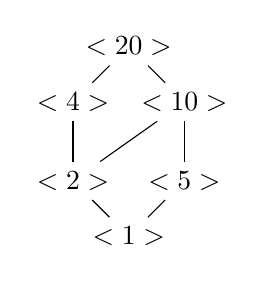
\begin{tikzpicture}[node distance=1cm]
			\node(20) {$<20>$};
			\node(10)  	[below right of=20] {$<10>$};
			\node(4)  	[below left of=20]  {$<4>$};
			\node(5) 	[below of=10] {$<5>$};
			\node(2)	[below of=4] {$<2>$};
			\node(1)	[below left of=5] {$<1>$};

			\draw(20) -- (10);
			\draw(20) -- (4);
			\draw(2) -- (4);
			\draw(2) -- (10);
			\draw(5) -- (10);
			\draw(2) -- (1);
			\draw(5) -- (1);
		\end{tikzpicture}
	\end{center}

	Here, the lines imply inclusion from top to bottom; that is
		\[<20>\subset<4>\subset<2>\subset<1>,\]
	for example. We won't spend a lot of time looking at subgroup lattices, but the idea of how to create them is more or less the same for our purposes.
\end{example}

Before we finish this section, we will look at some examples of groups and their subgroups.

\subsection*{The General Linear Group}
Numbers are just a small portion of the type of objects that sets can contain. One group that does not contain numbers is the General Linear Group, $(GL_{n}(\RR),\cdot)$, defined by
\[
	GL_{n}(\RR) = \left\{
	A=
	\left[
	\begin{array}{c c c c}
		a_{11} & a_{12} & \dots  & a_{1n} \\
		a_{21} & a_{22} & \dots  & a_{2n} \\
		\vdots & \vdots & \ddots & \vdots \\
		a_{n1} & a_{n2} & \dots  & a_{nn}
	\end{array}
	\right]
	:
	a_{i,j}\in\RR\text{ and } \det{(A)}\neq 0
	\right\}.
\]
In other words, it is the set of $n\times n$ invertible matrices with entries in $\RR$. The fact that every element in $GL_{n}(\RR)$ is invertible guarantees that inverses exist within the group. We know $I_{n}$ is contained within this group since its determinant is 1. Associativity is a little harder to prove, but it does indeed work. Hence, $GL_{n}(\RR)$ is in fact a group. The reason we point out this group is to mention one of its subgroups, the Special Linear Group $SL_{n}(\RR)$. We define this group by
\[
	\{A\in GL_{n}(\RR) : \det{(A)}=1\}.
\]
Let's show that $SL_{n}(\RR)$ is indeed a subgroup.

\begin{example}{Show $SL_{n}(\RR)$ is a subgroup.}
	We first need to find the identity within $SL_{n}(\RR)$. We know $\det{(I_{n})}=1$, so it lies within the Special Linear group. Next, we must verify that every element within $SL_{n}(\RR)$ has an inverse. Let $A\in SL_{n}(\RR)$. Then
	\[
		\det{(A^{-1})}=\det{(A)}^{-1}=1^{-1}=1,
	\]
	so the inverses exists within the subgroup. Finally, we must show that the group is closed. Let $A,B\in
	SL_{n}(\RR)$. Then
	\[
		\det{(AB)}=\det{(A)}\det{(B)}=1\cdot 1=1.
	\]
	Thus, we conclude that the group is closed, and therefore $SL_{n}(\RR)\leq GL_{n}(\RR)$
\end{example}

\subsection*{The Integers Multiplied by $n$}
We have seen that the group $\ZZ$ is a cyclic group generated by 1. It is true that there are other generators that generate subgroups of $\ZZ$ rather than $\ZZ$ itself. Specifically, we can take any $n\in\ZZ$ and examine the subgroup of $\ZZ$ generated by that element. We define this behavior with the notation
\[
	n\ZZ=\{nz:z\in\ZZ\} = <n>
\]
Our hope is that this forms a subgroup of $\ZZ$. It will turn out to be true, but let us look at a specific example.

\begin{example}{Consider the set $1727\ZZ$. Show that this is a subgroup of $\ZZ$, and that it is cyclic}
	Let's start with closure. Let $a,b\in 1727\ZZ$. Then $a=1727m$ and $b=1727n$ for some $n,m\in\ZZ$. Therefore
	\[
		a+b=1727m+1727n= 1727(m+n)\in 1727\ZZ,
	\]
	so $1727\ZZ$ is closed. We know the identity is inside of $1727\ZZ$ since $1727\cdot 0=0$. Finally, we need inverses to be inside the subgroup. Let $a\in 1727\ZZ$. Then
	\[
		a+-a= 1727n + (-1727n) = 0.
	\]
	from \cref{thm:cyclic_subgroup}, we know that it is cyclic since $\ZZ$ is cyclic.
\end{example}
The notion of multiplication of a group and an element of the group is a very important topic that we will discuss later.

\subsection*{The Center of a Group}
The next subgroup we will look at is called the center of a group. Recall that nowhere in the definition of group is it stated that the operation is commutative. To take care of this issue, we define a special subgroup called the center of a group. The formal definition is as follows.
\begin{definition}{Center of a Group}
	Let $G$ be a group. The center of $G$ is the group
	\[
		Z(G)=\{z\in G : zg=gz\ \forall g\in G\}.
	\]
	That is, the center of a group is the set of all elements that commute within $G$.
\end{definition}
It follows that if $G$ is an abelian group, then $Z(G)=G$. We claim that this is a subgroup.
\begin{example}{Show $Z(G)\leq G$}
	The identity is in the center since $eg = ge\ \forall g\in G$. Inverses require a little more work. Let $z\in Z(G)$. We need $z^{-1}g=gz^{-1}\ \forall g\in G$. Consider
	\begin{align*}
		zg         & =gz                \\
		z^{-1}(zg) & = z^{-1}(gz)       \\
		(z^{-1}z)g & = (z^{-1}g)z       \\
		g          & = (z^{-1}g)z       \\
		gz^{-1}    & = (z^{-1}g)zz^{-1} \\
		gz^{-1}    & = z^{-1}g.
	\end{align*}
	This is exactly what we needed, so we conclude that the group contains inverses. We will leave closure to you.
\end{example}
